\documentclass[letterpaper,12pt]{article}

\usepackage{listings}
\usepackage{hyperref}
\usepackage{graphicx}
\usepackage{ulem}
\usepackage{geometry}
\usepackage{amssymb}

\lstdefinestyle{code}{
	basicstyle=\ttfamily\small
}

\lstset{style=code}

\graphicspath{ {./figures/} }

\geometry{
	letterpaper,
	top=2.54cm,
	bottom=2.54cm,
	left=2.54cm,
	right=2.54cm
}

\begin{document}
\title{Complex Codomain Coloring, the Mandlebrot Set, and Primes}
\author{Jake Looney\\ Undergrad at the University of Tennessee Knoxville}
\date{January - March, 2022}
\maketitle

\pagenumbering{roman}
\tableofcontents
\newpage
\pagenumbering{arabic}

\section{Motivation}
Let $f:\mathbb{C}\rightarrow\mathbb{C}$ be a function from the complex plane to itself.
The standard, practical way to visually represent $f$ is with \textit{domain coloring}, whereby you take a region
on the complex plane, apply the function to a grid a points within that region, and color each pixel based on the output of those points.
This, in effect, shows you where "each point goes" after applying the function. However, what if you want to see
where "each point is from"? To do that, we use \textit{codomain coloring}, which is the concern of this paper.
Codomain coloring works by taking a large set of points, applying the function to each point,
and then storing each output point with its corresponding input point. Then, you select a region on the plane,
divide that region into a grid, and color each pixel based on the \textit{input point} of the nearest \textit{output point}.
In metaphor, it is like giving each point a name, having those points move around the plane, and then coloring pixels based off
the name of the closest point.
There's not many reasons to do this: it goes against the standard, its computationally intensive, slow as all get out, blocky, imprecise, and only shows one point for each pixel.
However, despite this, I did discover something pretty interesting while shoving fun functions into it. But first, an explanation of the code.

\section{Code explanation}
There is an attached GitHub repository containing the code. You can view it here: \url{https://github.com/6a6c/jraph} \\

The function \verb|createPicture| takes a map of pixel indices and complex points to output a bitmap image.
It mainily utiliizes a bitmap implementation I stole from one of my classes,
but importantly it colors points in the image based on their argument and magnitude:
\begin{lstlisting}[language=c++]
    z = fit->second;
    mag = abs(z);
    ar = arg(z);

    pixarray[fit->first].red = min(5*mag, 255.0);
    pixarray[fit->first].blue = min(40*ar, 255.0);
    pixarray[fit->first].green = min(100*mag, 255.0);
\end{lstlisting}
This can be changed in order to alter the colorscheme.\\

There are three main functions that are used to create these graphs. The function \verb|makeFunction| creaates a multimap of doubles corresponding to output magnitudes and a pair of complex points corresponding to input and output points of a function. To do this, it applies a function to a region of complex points and adds them to the multimap:
\begin{lstlisting}[language=c++]
for( i = -1 * pts; i < pts; i++){
  for( j = -1 * pts; j < pts; j++){

    z = complex<double>(aCoeff * i * i * i, aCoeff * j * j * j);

    output = func(z);

    // if(abs(output) > 2) continue;

    function->insert(make_pair(abs(output), make_pair(output, z)));
  }
}
\end{lstlisting}
The points selected to be input points for the function are scaled based on a cubic function.
This means that there are more points around 0 (the interesting parts) and less points further out.
The coefficient on the cubic as well as the number of points can be changed.
The output is set to the \verb|func| function, which can be altered to change the function. Note, the commented out line, which
will ignore points that diverge to infinity when calculating the Mandlebrot function. This will help keep the map small and runtime down. \\

The function \verb|makeMap| is used to create the maps that are passed to \verb|createPicture|.
To do this, it is passed a multimap created by \verb|makeFunction| as well as the boundaries of a region on the complex plane.
It inserts points into the map based on their preimage by passing points to \verb|preImage| based on the region.
\begin{lstlisting}[language=c++]
for(i = 0; i < w * h; i++){
  complex<double> z(realLeft + ((i\%w) * ((realRight - realLeft)/w)),
			imagTop - ((i/w) * ((imagTop - imagBot)/h)));

  complex<double> pre = preImage(z, function);

  ret->insert(make_pair(i, pre));

}
\end{lstlisting}
\verb|preImage| works by first isolating a range of the function multimap with magnitudes within a certain ammount of the image point z.
Then, it iterates through this range and finds the point with the least distance from z.
The input point that corresponds to this output point (that is, second part of the pair in the multimap).

\begin{lstlisting}[language=c++]
double mag = abs(z);
double d1, d2, best;
map< double, pair< complex<double>, complex<double> >
    >::const_iterator low, high, fit, bit;
size_t i = 0;

low = func->lower_bound(mag-(ep * mag));
high = func->upper_bound(mag+(ep * mag));

bit = low;
best = 100000;
for(fit = low; fit != high; fit++){
  d1 = sqrt( pow(z.real() - fit->second.first.real(), 2) +
       pow(z.imag() - fit->second.first.imag(), 2) );

  if(d1 < best) {
    best = d1;
    bit = fit;
  }

}

return bit->second.second;

\end{lstlisting}

The result, after calling \verb|preImage| on all the points for the picture, is a preimage point for each point in the codomain. \\ \\

\section{That's cool, but what do the pictures look like?}

For reference, it's important to see what the unaltered complex plane looks like:

\begin{figure}[h]
	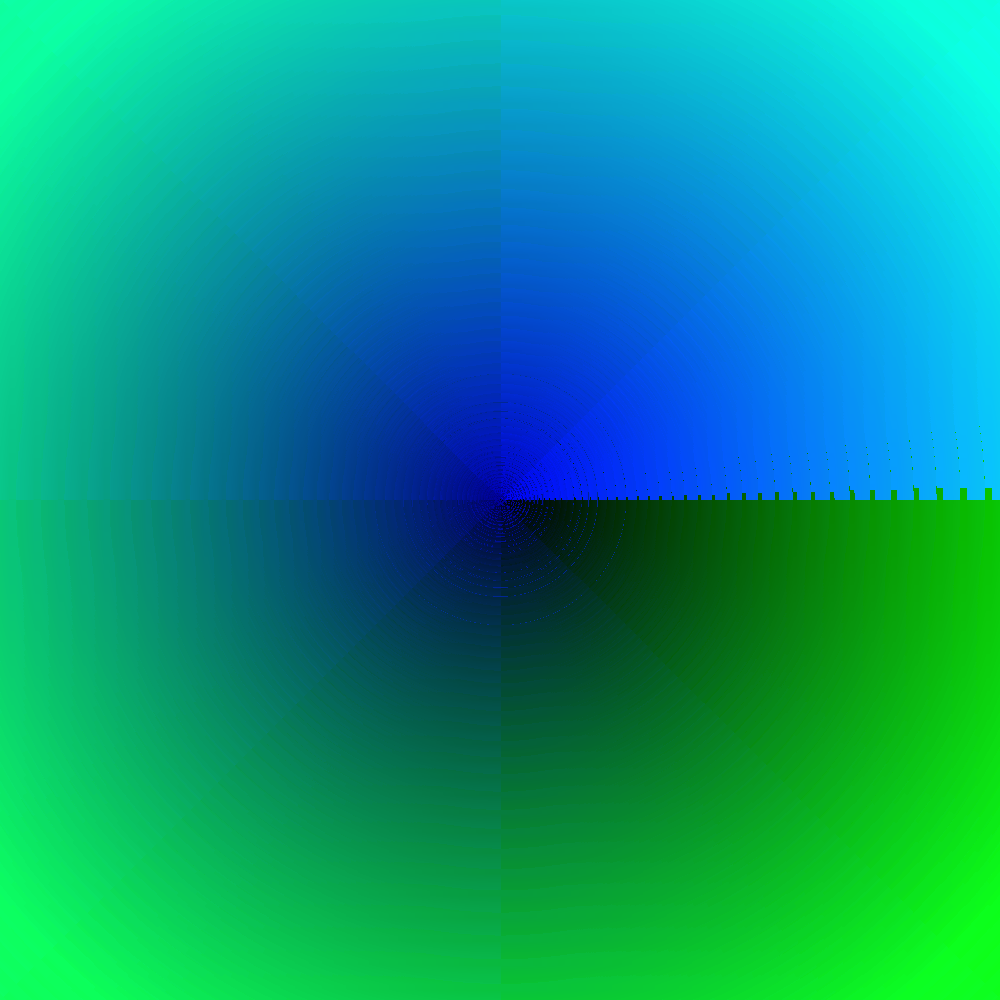
\includegraphics[width=8cm]{f(z)=z}
	\centering
	\caption{\small$f(z) = z$}
	\centering
\end{figure}

This image was obtained by using $f(z) = z$ as the function through the codomain grapher.
The real and imaginary axes runs directly through the middle.
Because all points in the domain this function equal their outputs in the codomain, this graph can be used as the domain for other functions.
\\
Also, notice here some of the limitations in this method in the artifacts the graph produces.
Near the positive real axis, there are some instances of the green "jumping up" into the first quadrant.
\todo{Find out why this is and describe it}
\\
Here's another example of the codomain grapher:

\begin{figure}[h]
	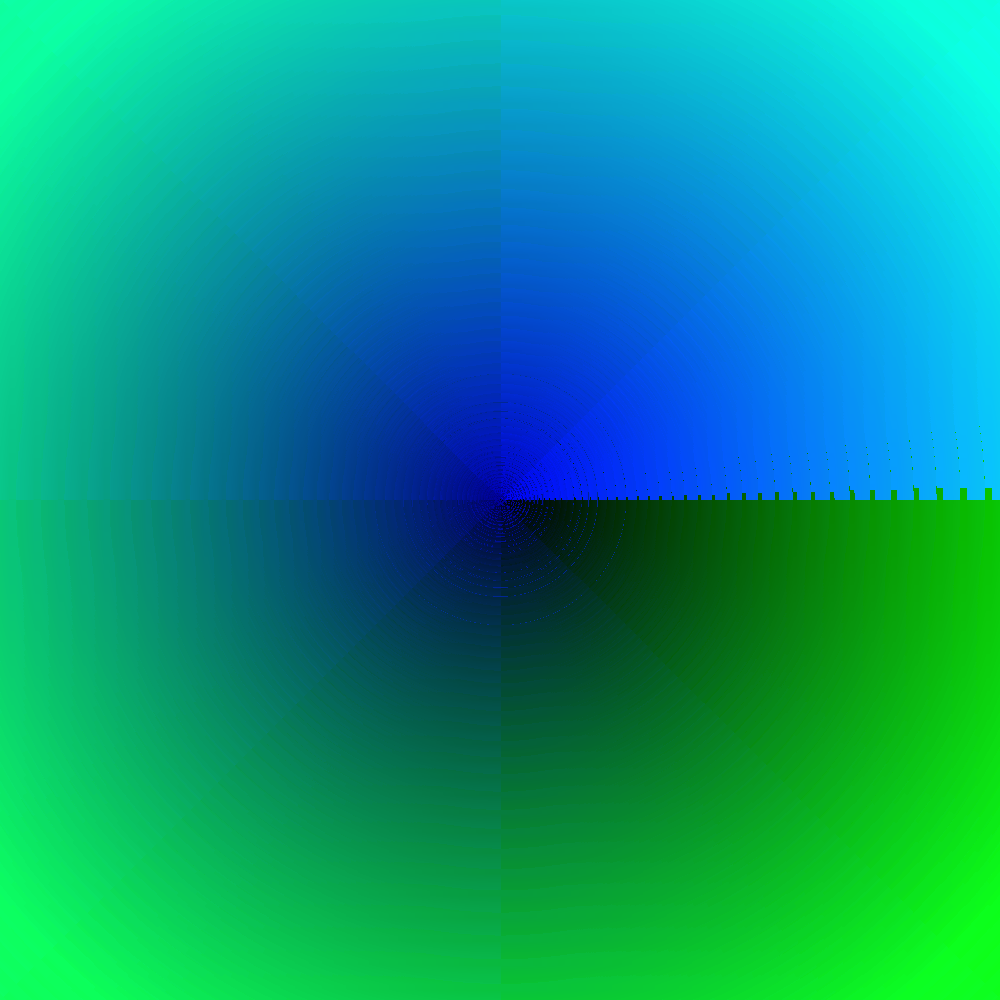
\includegraphics[width=6cm]{f(z)=z}
	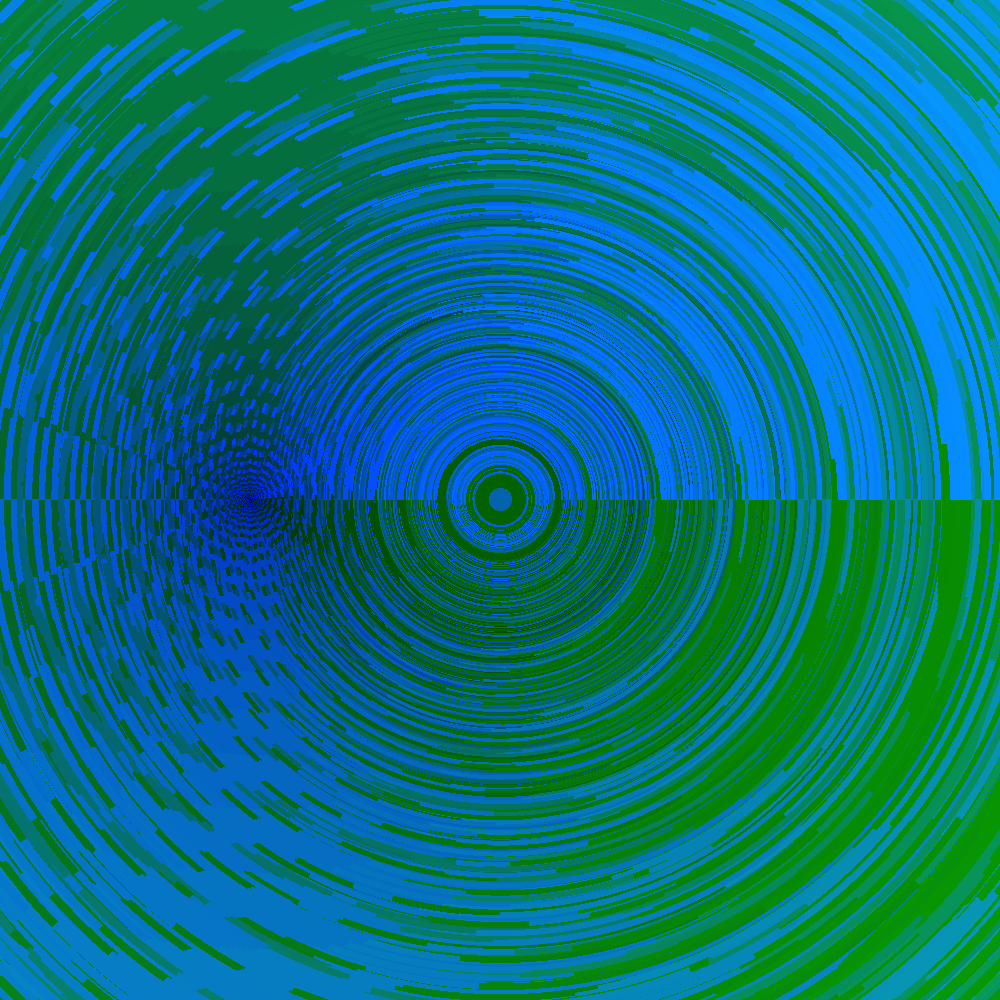
\includegraphics[width=6cm]{f(z)=z^3-1}
	\centering
	\caption[\small]{The complex plane before and after applying $f(z) = z^3 - 1$}
	\centering
\end{figure}

This is the function $f(z) = z^3 - 1$. Compare this function with it's corresponding domain graph:

\begin{figure}[h]
	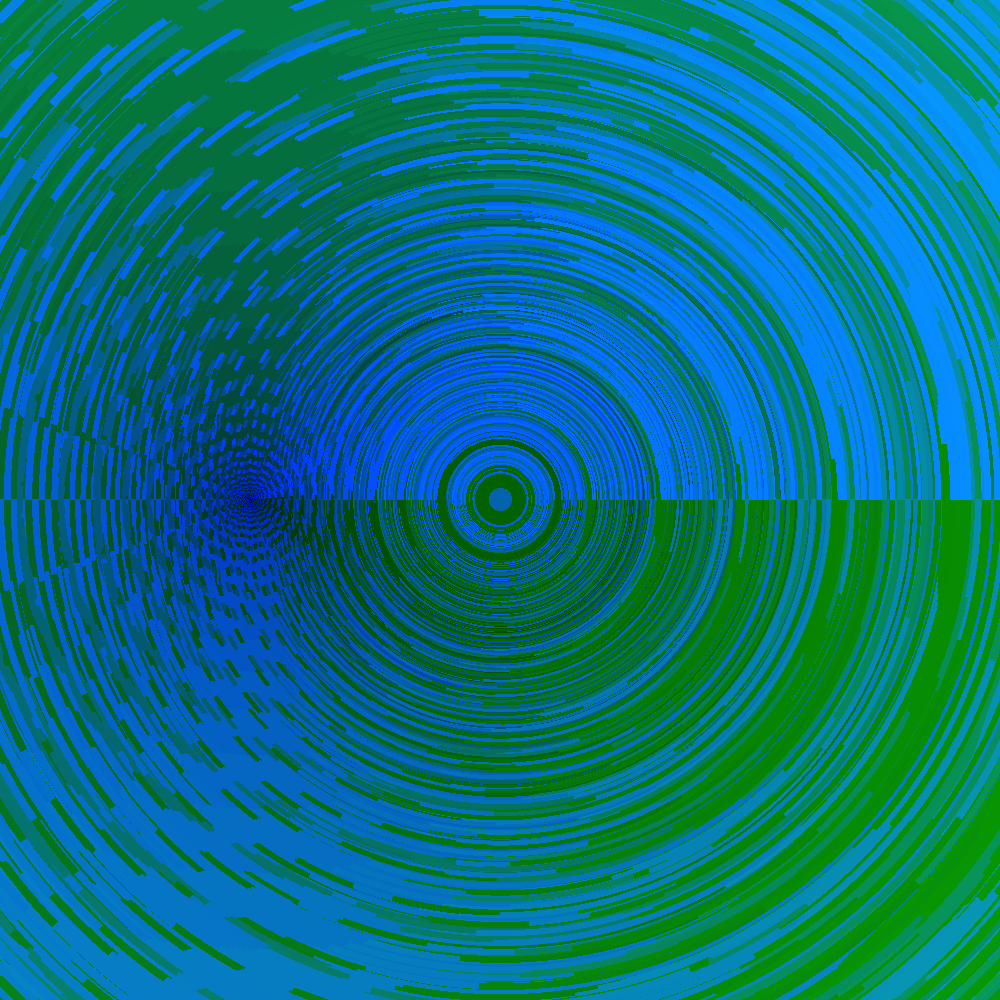
\includegraphics[width=6cm]{f(z)=z^3-1}
	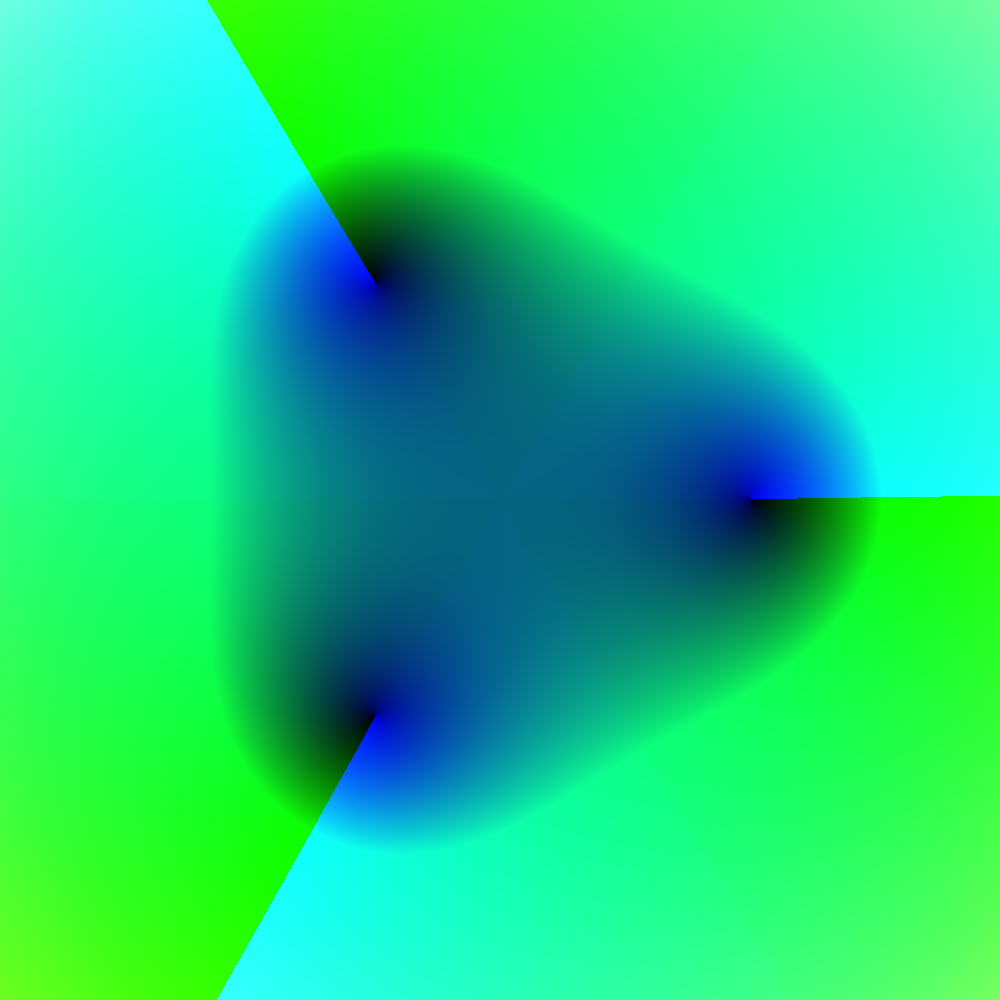
\includegraphics[width=6cm]{f(z)=z^3-1_D}
	\centering
	\caption[basicstyle=\small]{The codomain graph(left) and domain graph(right) of $f(z) = z^3 - 1$}
\end{figure}

Both graphs show the same interval on the complex plane, but one shows where points in that interval go and one shows some points that end up in that interval.
This highlights the biggest practical restriction with this method of graphing: points in the codomain only display one preimage point despite potentially having more preimage points.
For intance, we can clearly see from the domain graph that this function has 3 roots.
However, as each point can only be colored once, 0 only shows the value of the root $z= \frac{-1 + i\sqrt{3}}{2} = -0.5000 + 0.8660i$, omitting the other two roots. \\

I hope these examples illustrate how to interpret these graphs.
After trying with a normal functions, the obvious next step was:

\section{Jamming the Mandlebrot function in this}

To graph the Mandlebrot with the codomain grapher, one only needs to use points with a magnitude to less than two to genereate the function.
Anypoints with a magnitude of greater than two will diverge to infinity and will not be apart of the set$^{[citation needed]}$.
So, to genereate the collection of Mandlebrot graphs, I set pts to 2000 and the aCoeff to $10^{-9}$

In addition to this, most images shown are on the inteveral $ -0.5 \leq Re(z), Im(z) \leq 0.5$.
This is because this is the pretty and interesting part and everything else is just kinda circles.

Let's take a look at the first one of these I tried, using 500 iterations before bailing out of the Mandlebrot function:

\begin{figure}[h]
	\noindent\makebox[\textwidth]{%
		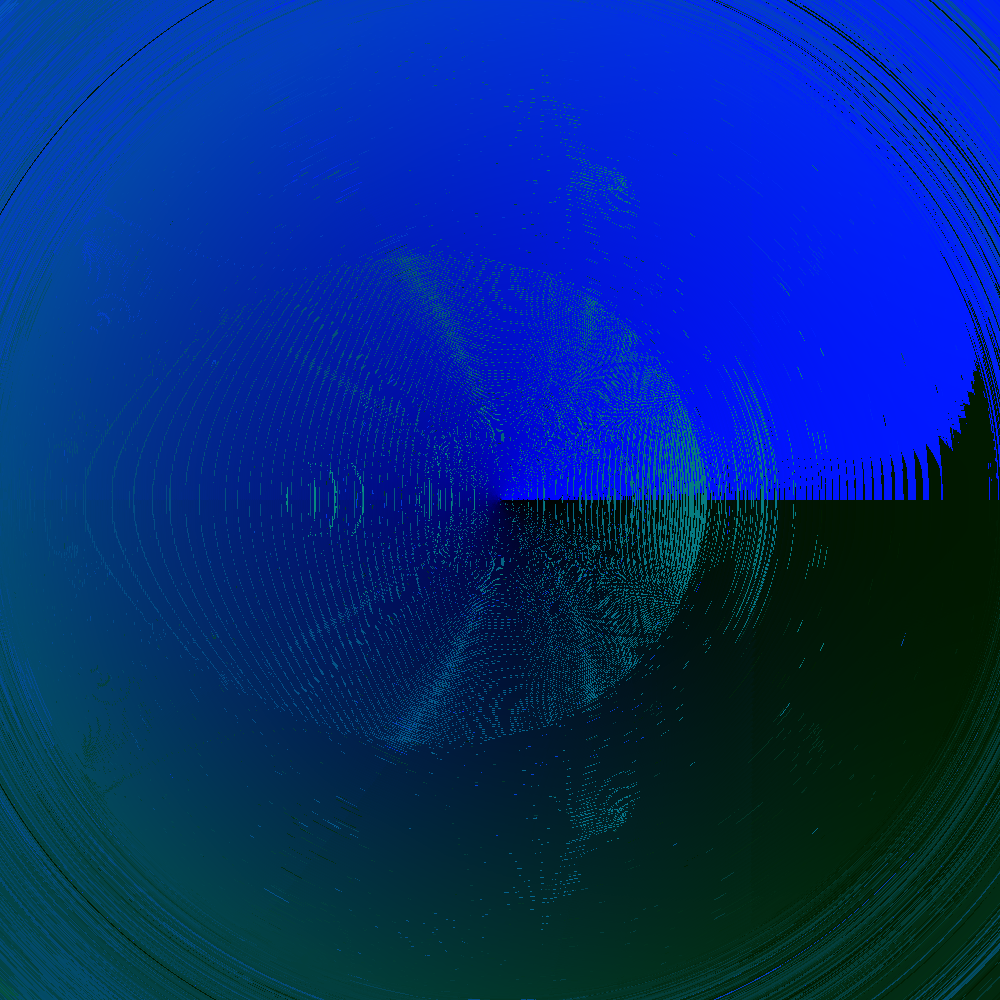
\includegraphics[width=8cm]{500iter}}
	\centering
	\caption{500 iterations}
	\centering
\end{figure}

Wowie ain't that cool! Lets do that again but this time, we'll edit the interval and image size so that it makes a good desktop wallpaper:
\pagebreak
\begin{figure}[h]
	\noindent\makebox[\textwidth]{%
		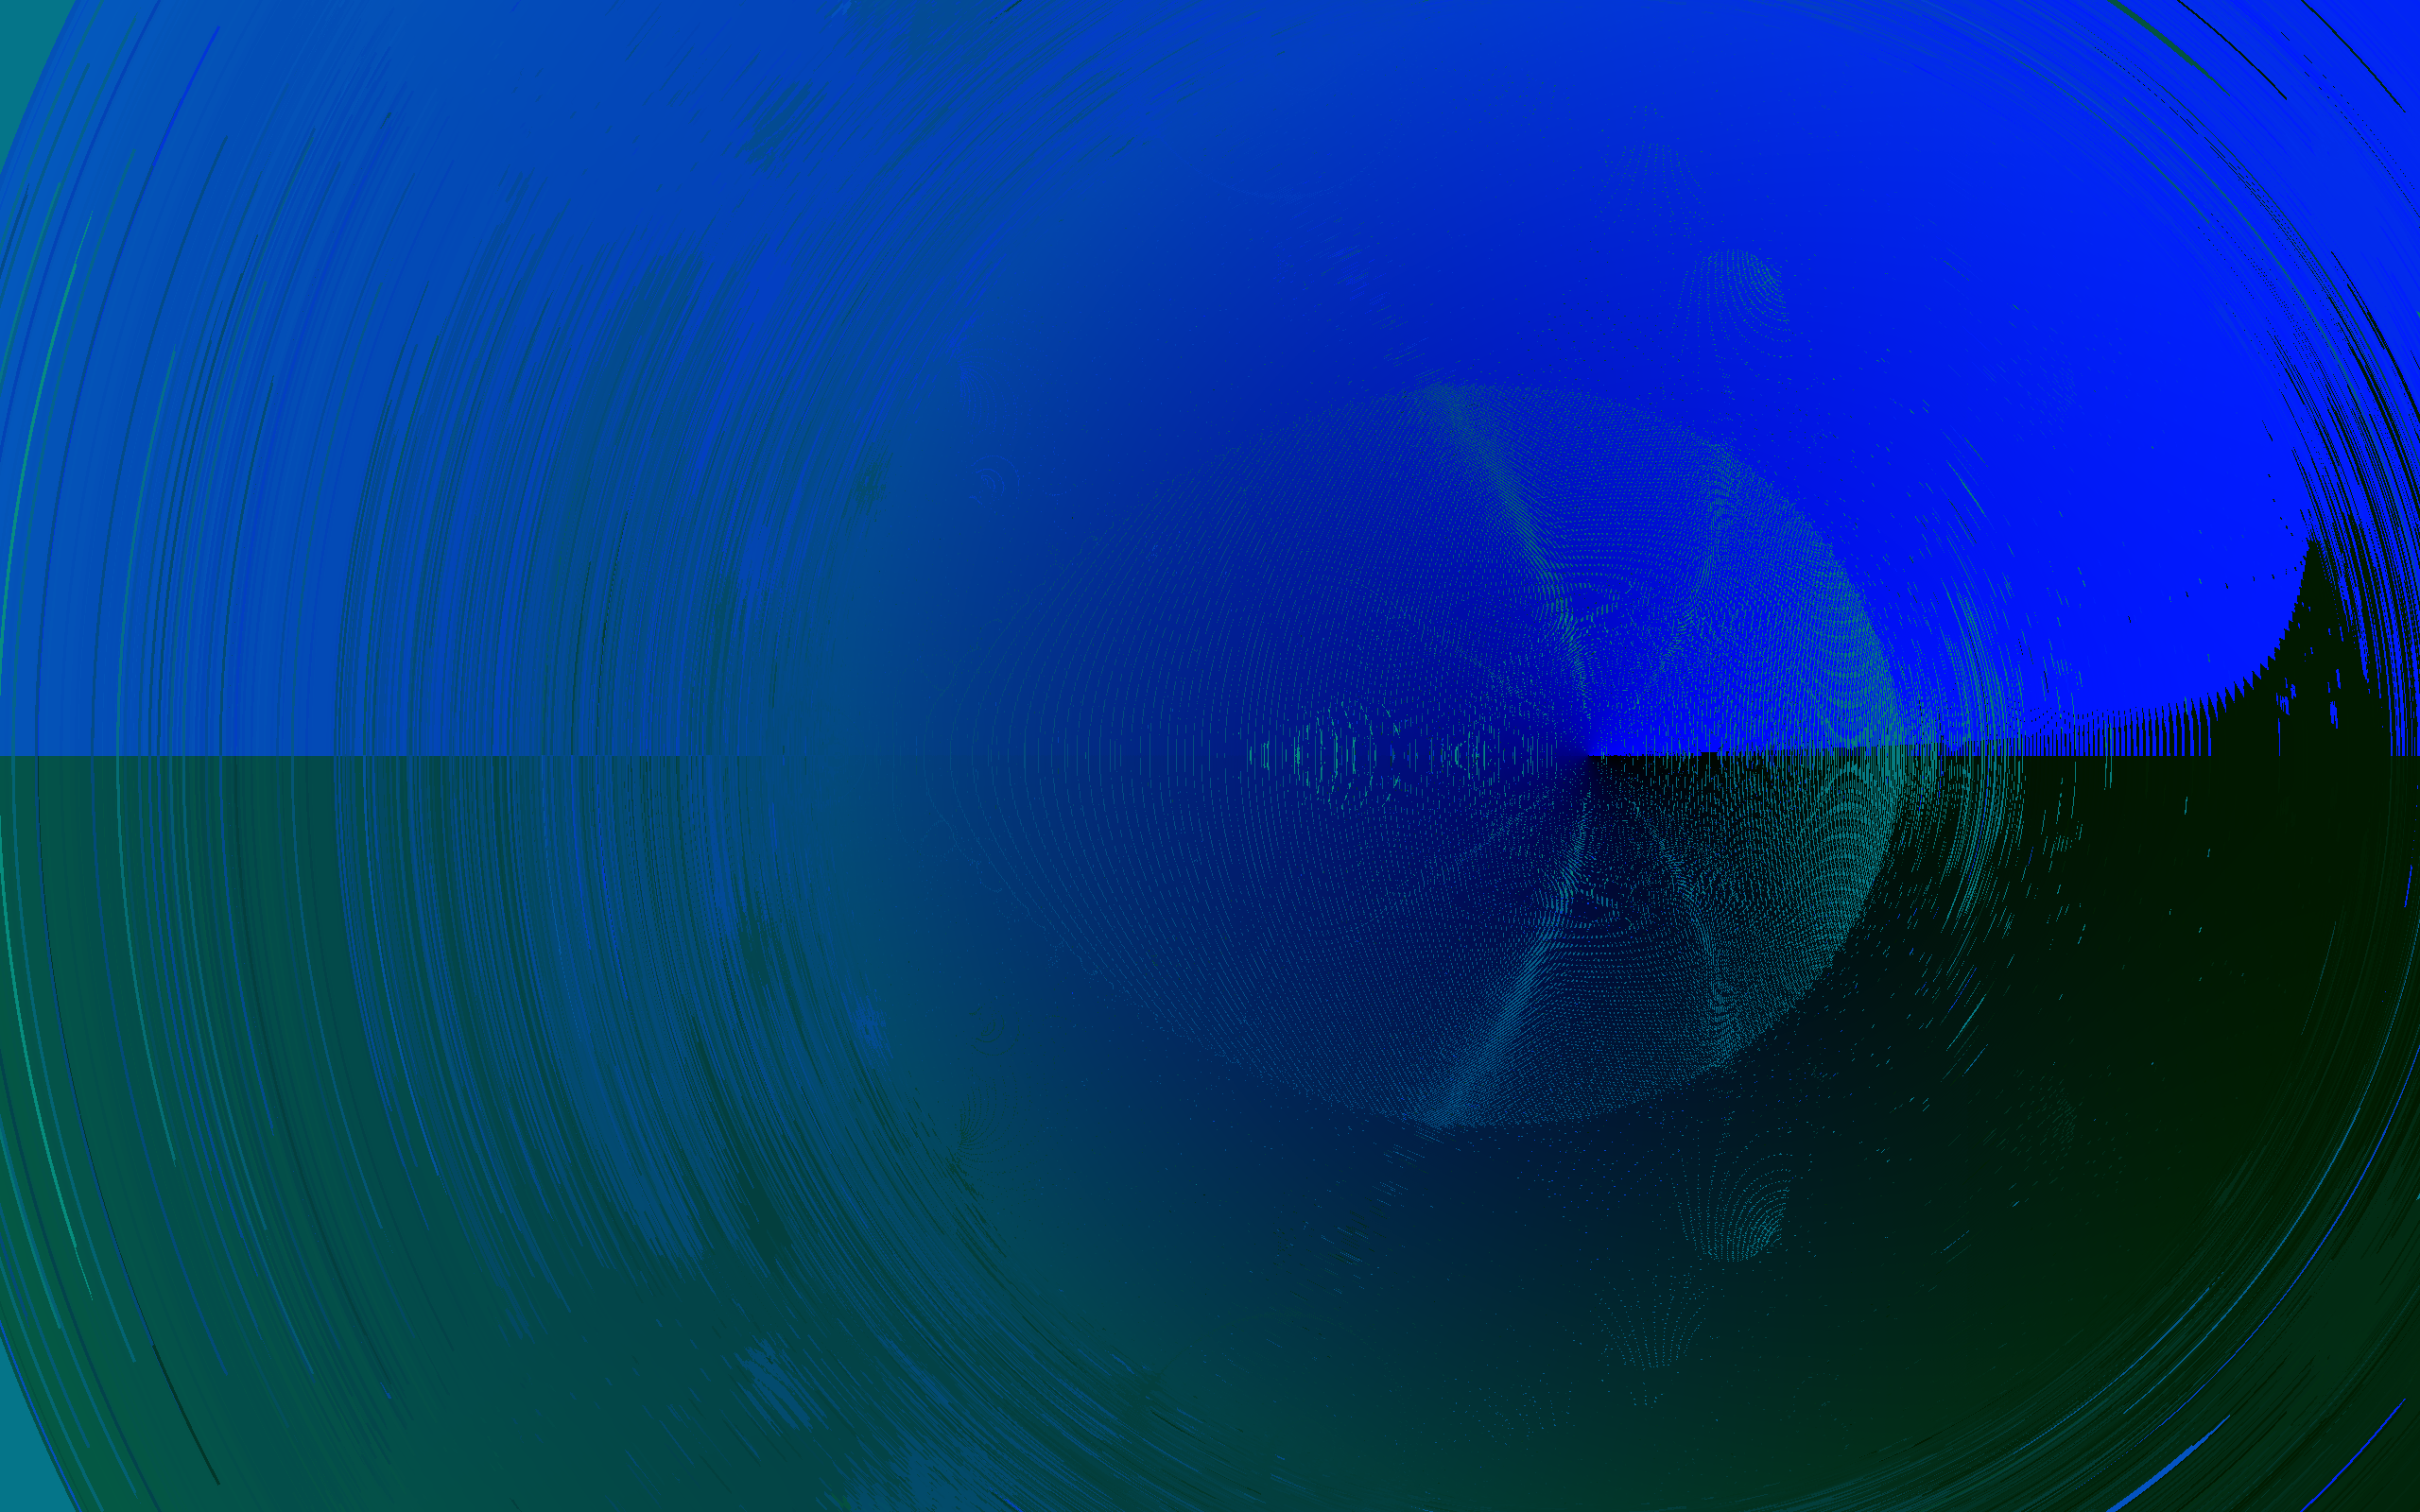
\includegraphics[width=14cm]{mandoback}}
	\centering
	\caption{A bitching wallpaper, send it to your colleagues!}
	\centering
\end{figure}

Wow that's nice. I was really suprised at the detail that shows up.
I almost walked away from it but then I remebered that points in iterative functions iterate. So I tried changing the number of iterations:

\begin{figure}[h]
	\noindent\makebox[\textwidth]{%
	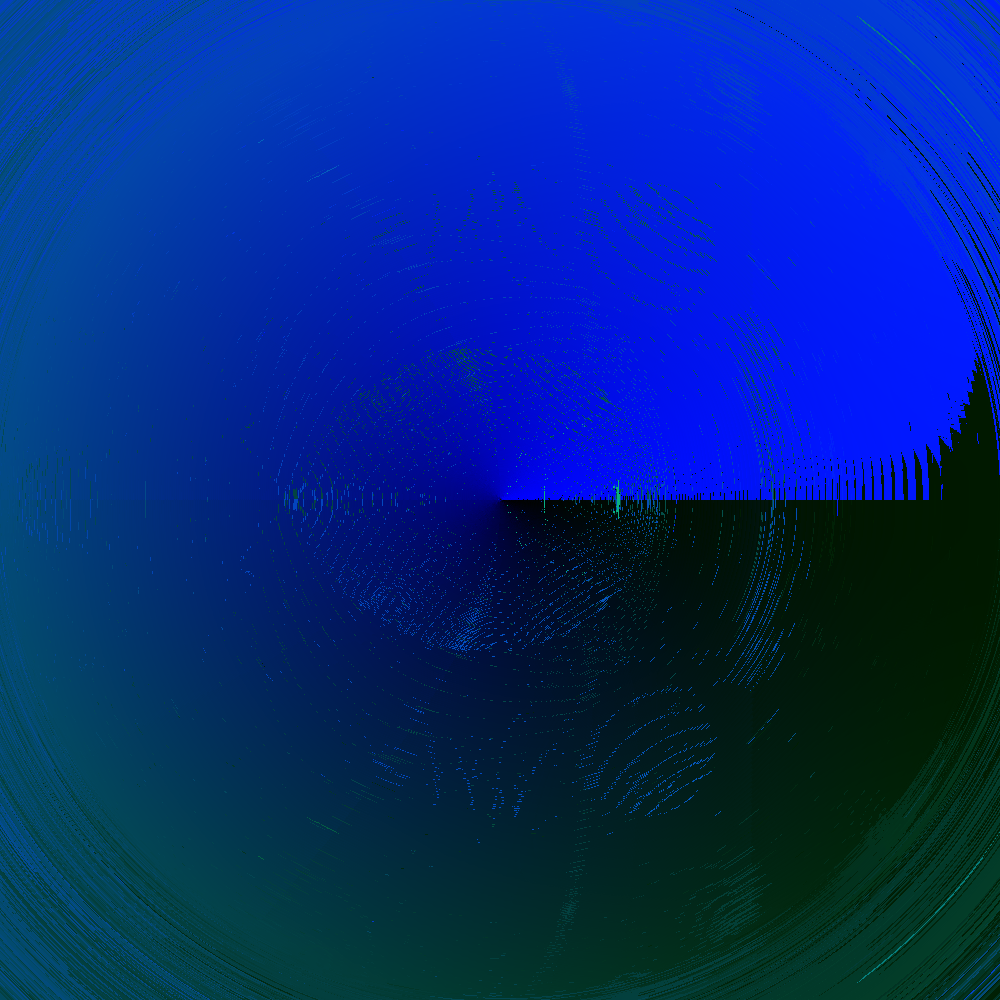
\includegraphics[width=5.5cm]{501iter}
	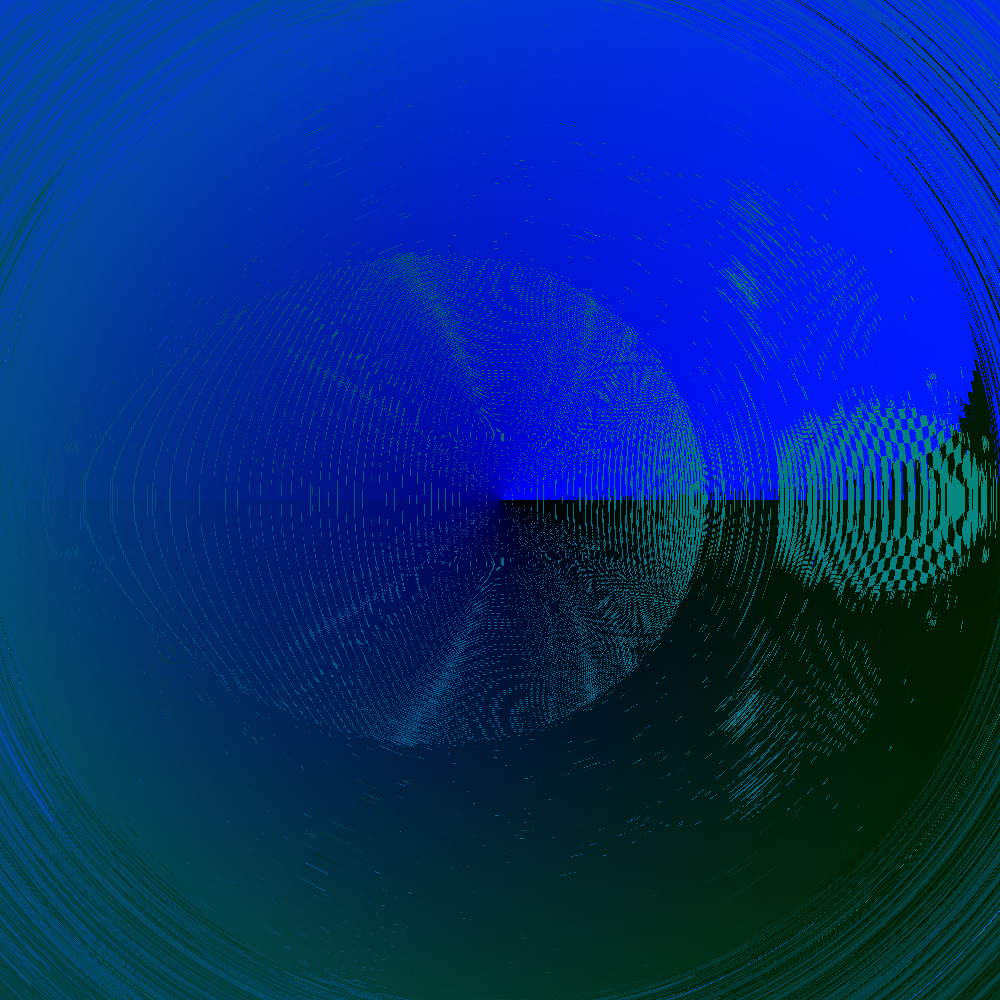
\includegraphics[width=5.5cm]{502iter}
	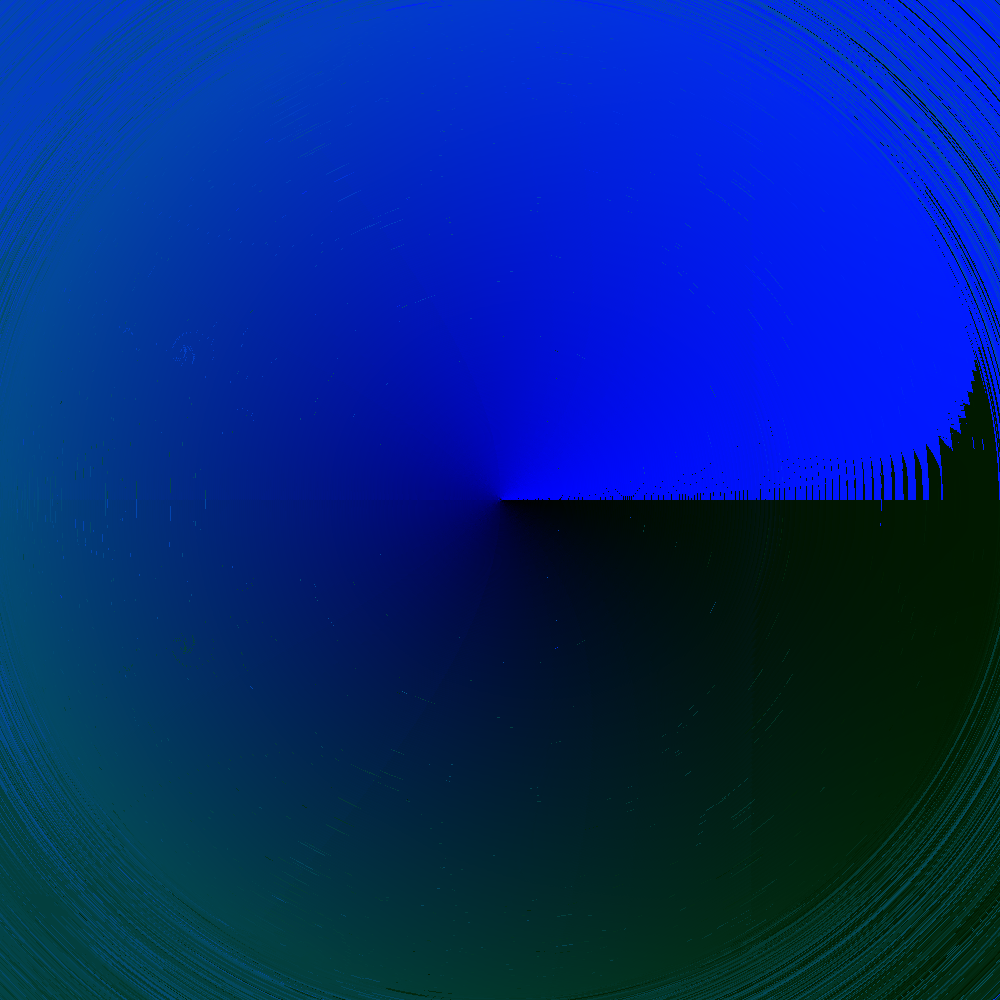
\includegraphics[width=5.5cm]{503iter}}
	\centering
	\caption{LtR: 501 iterations, 502 iterations, and 503 iterations}
\end{figure}

Oh wow that's cool. 501 has some detail but is nothing like 500. 502 looks exactly like 500 but with an extra little thingy on the right of it.
503 has basically no detail though. Wait a second...

\section{Ding dong, get the door, its the motherfucking prime numbers!}

Yoooooooooo!!!!!!\\
Alright, so. For any numbers, less than 50 (and really up until 100), there's too much noise for the patterns to shine.
Primes under 50 in particular are less distinct from composite numbers because some of the numbers "haven't gotten out of the way yet".
However, over 50, primes iterations are distinguishable by their lack of detail, where detail is defined here to be "how pretty and interesting the picture looks".


\end{document}
